%
% naeherungsbrueche.tex
%
% (c) 2020 Prof Dr Andreas Müller, Hochschule Rapperswil
%
\subsection{Näherungsbrüche\label{subsection:cf:naherungsbrueche}}
In den Beispielen in Abschnitt~\ref{subsection:cf:beispiele} haben
wir kein Beispiel gerechnet, in dem wir einen Kettenbruch in einen
gewöhnlichen Bruch umgerechnet haben.

\subsubsection{Einen Kettenbruch in einen gewöhnlichen Bruch umwandeln}
Selbstverständlich kann man einen Kettenbruch in einen gewöhnlichen
Bruch umwandeln:
\begin{align*}
2+\cfrac{1}{
3+\cfrac{1}{
1+\cfrac{1}{5}}}
&=
2+\cfrac{1}{
3+\cfrac{5}{11}}
=
1+\cfrac{11}{38}
=
\cfrac{49}{38}.
\end{align*}
Man beginnt also beim ``untersten'' Bruch, macht die Summanden gleichnamig,
bildet den Kehrwert und so weiter, bis man ``ganz oben'' angekommen ist.
Wenn man mit diesem Vorgehen immer länger werdende Kettenbrüche wie
$[1;2], [1;2,3], [1;2,3,4],\ldots$ in gewöhnliche Brüche umwandeln soll,
dann muss man immer wieder von vorne beginnen, weil der ``unterste Bruch''
jedesmal anders ist.
Das Ziel muss daher sein ein Verfahren zu entwickeln, welches die Berechnung
der Brüche ``von oben nach unten'' ermöglicht.

\subsubsection{Naherungsbrüche}
Um den Wert eines unendlichen Kettenbruchs zu bestimmen, muss man den
Bruch nach einer endlichen Anzahl von Brüchen abbrechen und in einen
gewöhnlichen Bruch umwandeln.
Wir nennen daher
\[
\frac{p_n}{q_n}
=
a_0+\cfrac{b_1}{
a_1+\cfrac{b_2}{
a_2+\cfrac{b_3}{
a_3+\cfrac{b_5}{
\dots+
\cfrac{b_{n-1}}{
a_{n-1}+\cfrac{b_n}{a_n}
}}}}}
\]
den $n$-ten Näherungsbruch des Kettenbruches $[a_0,a_1,a_2,\dots]$.
Der Wert des Kettenbruchs ist dann der Grenzwert
\[
[a_0;a_1,a_2,a_3,\dots]
=
\lim_{n\to\infty}\frac{p_n}{q_n}.
\]
Damit man diesen Grenzwert effizient berechnen kann, wäre hilfreich,
wenn man $p_{n+1}$ und $q_{n+1}$ aus $p_n$ und $q_n$ bestimmen könnte.

\subsubsection{Matrixnotation}
Die Werte der Brüche $p_n/q_n$ interessieren uns nicht so sehr wie
die Zahlen $p_n$ und $q_n$ selbst.
Es ist daher sinnvoll, diese nicht als Bruch sondern als Vektor
\[
v_n = \begin{pmatrix} p_n\\q_n\end{pmatrix}
\]
zu behandeln.
Gesucht ist dann eine Abbildung, die aus dem Vektor $v_n$ den Vektor
$v_{n+1}$ macht.
Mit so einer Abbildung kann man die Näherungsbrüche schrittweise
von links nach rechts aufbauen:
\[
v_0 =\begin{pmatrix}a_0\\1\end{pmatrix}
\rightarrow
v_1
\rightarrow
v_2
\rightarrow
\dots
\rightarrow
v_{n}
\rightarrow
v_{n+1}
\rightarrow
\dots
\]
Wenn die Abbildung durch Multiplikation mit Matrizen realisiert werden
kann, dann kann man wegen der Assoziativität des Matrizenproduktes
die Anwendungsreihenfolge auch umkehren und damit die Folge von rechts
nach links konstruieren.

Für die Auflösung eines Kettenbruchs muss man einen Bruch der Form
\[
\frac{b_1}{a_1+\cfrac{b_2}{a_2}}
=
\frac{b_1}{\frac{a_1q_2+b_2}{a_2}}
=
\frac{b_1a_2}{a_1a_2+b_2}
\]
in einen gewöhnlichen Bruch umwandeln können.
Ausserdem muss dies in Vektorform geschrieben werden können.
Tatsächlich ist
\begin{equation}
\begin{pmatrix}
b_1q\\
a_1a_2+b_2
\end{pmatrix}
=
\begin{pmatrix}
0&b_1\\
1&a_1
\end{pmatrix}
\begin{pmatrix}
b_2\\a_2
\end{pmatrix}.
\label{eqn:cf:matrixdef}
\end{equation}
Wir kürzen die Matrix in \eqref{eqn:cf:matrixdef} im Folgenden
mit $N(b_1,a_1)$.
Die Asymmetrie zwischen $a_1,b_1$ und $a_2,b_2$ kann verbessert werden, 
wenn man auch den Faktor für den Bruch $b_2/a_2$ als Matrix schreibt.
Man erhält dann
\[
N(b_1,a_1)
N(b_2,a_2)
=
\begin{pmatrix}
0&b_1\\
1&a_1
\end{pmatrix}
\begin{pmatrix}
0&b_2\\
1&a_2
\end{pmatrix}
=
\begin{pmatrix}
b_1&b_1a_2    \\
a_1&a_1a_2+b_2
\end{pmatrix}
=
\begin{pmatrix}
p_1&p_2\\
q_1&q_2
\end{pmatrix}.
\]
Fügt man im letzten Nenner den nächsten Bruch $b_3/a_3$ hinzu, erhält man
die Brüche in Matrixdarstellung
\[
N(b_1,a_1)
N(b_2,a_2)
N(b_3,a_3)
\dots
N(b_{n+1},a_{n+1})
N(b_n,a_n)
=
\begin{pmatrix}
0&b_1\\
1&a_1
\end{pmatrix}
\begin{pmatrix}
0&b_2\\
1&a_2
\end{pmatrix}
\begin{pmatrix}
0&b_3\\
1&a_3
\end{pmatrix}
=
\begin{pmatrix}
p_2&p_3\\
q_2&q_3
\end{pmatrix}
\]
für die Näherungsbrüche des Kettenbruchs
\[
x
=
\cfrac{b_1}{
a_1+\cfrac{b_2}{
a_2+\cfrac{b_3}{a_3}}}
=
\frac{p_3}{q_3}.
\]
Die Matrixnotation ermöglich also, von einem beliebig langen Kettenbruch
mit $a_0=0$ die Näherungsbrüche zu bestimmen.
Es gilt
\begin{equation}
\begin{pmatrix}
0&b_1\\
1&a_1
\end{pmatrix}
\begin{pmatrix}
0&b_2\\
1&a_2
\end{pmatrix}
\begin{pmatrix}
0&b_3\\
1&a_3
\end{pmatrix}
\dots
\begin{pmatrix}
0&b_{n-1}\\
1&a_{n-1}
\end{pmatrix}
\begin{pmatrix}
0&b_{n}\\
1&a_{n}
\end{pmatrix}
=
\begin{pmatrix}
p_{n-1}&p_n\\
q_{n-1}&q_n
\end{pmatrix}.
\label{eqn:cf:matrixentwicklung}
\end{equation}
Der Vorteil dieser Schreibweise ist, dass das Matrizenprodukt
dank dessen Assoziativität sowohl von
links als auch von rechts her ausmultipliziert werden kann.

Im Produkt \eqref{eqn:cf:matrixentwicklung} fehlt $a_0$.
Gesucht ist daher eine Matrix, mit der man die Addition eines weiteren
Terms ausdrücken könnte.
Eine solche Matrix müsste auch nützlich sein, um die bisher verwendeten
Matrizen $N(b_i,a_i)$ aufzubauen.
Aus der Perspektive der Näherungsbrüche setze sich $N(b_1,a_1)$ 
zusammen aus zwei Schritten, nämlich zunächst die Addition von $a_1$
zum Bruch $b_2/a_2$ gefolgt von der Division von $b_2$ durch das Resultat
der Addition.
Es sollte also Matrizen $A(a_1)$ und $Q(b_1)$ geben, die dies vollziehen.
\begin{align*}
a_1+\frac{b_2}{a_2}
&=
\frac{a_1a_2+b_2}{a_2}
&&\Rightarrow
&
\begin{pmatrix}
a_1a_2+b_2\\
a_2
\end{pmatrix}
&=
\begin{pmatrix}
1&a_1\\
0&1
\end{pmatrix}
\begin{pmatrix}
b_2\\
a_2
\end{pmatrix}
=
A(a_1)
\begin{pmatrix}
b_2\\
a_2
\end{pmatrix}
\\
\frac{b_1}{\frac{p}{q}}
&=
\frac{qb_1}{p}
&&\Rightarrow
&
\begin{pmatrix}
qb_1\\
p
\end{pmatrix}
&=
\begin{pmatrix}
0&b_1\\
1&0
\end{pmatrix}
\begin{pmatrix}
p\\
q
\end{pmatrix}
=
Q(b_1)
\begin{pmatrix}
p\\
q
\end{pmatrix}
\end{align*}
Die Matrix $N(b_1,a_1)$ lässt sich jetzt aus $A(a_1)$ und $Q(b_1)$ 
zusammensetzen, denn
\begin{equation}
Q(b_1)
A(a_1)
=
\begin{pmatrix}
0&b_1\\
1&0
\end{pmatrix}
\begin{pmatrix}
1&a_1\\
0&1
\end{pmatrix}
=
\begin{pmatrix}
0&b_1\\
1&a_1
\end{pmatrix}
=
N(b_1,a_1).
\label{eqn:cf:faktorisierung}
\end{equation}

Die Faktorisierung \eqref{eqn:cf:faktorisierung} ermöglicht den Aufbau
der Näherungsbrüche in \eqref{eqn:cf:matrixentwicklung} noch weiter
zu zerlegen in das Produkt
\begin{align}
\begin{pmatrix}
p_{n-1}&p_n\\
q_{n-1}&q_n
\end{pmatrix}
&=
N(b_1,a_1)
N(b_2,a_2)
\cdots
N(b_{n-1},a_{n-1})
N(b_n,a_n)
\notag
\\
&=
Q(b_1)
A(a_1)
Q(b_2)
A(a_2)
\cdots
Q(b_{n-1})
A(a_{n-1})
Q(b_{n})
A(a_{n})
\label{eqn:cf:faktorisierung2}
\end{align}
für einen Kettenbruch mit $a_0=0$. 
Für einen beliebigen Kettenbruch mit $a_0$ muss das Produkt von links
mit $A(a_0)$ multipliziert werden.
Tatsächlich ist
\begin{align*}
A(a_0)
\begin{pmatrix}
p_{n-1}&p_n\\
q_{n-1}&q_n
\end{pmatrix}
=
\begin{pmatrix}
1&a_0\\
0&1
\end{pmatrix}
\begin{pmatrix}
p_{n-1}&p_n\\
q_{n-1}&q_n
\end{pmatrix}
=
\begin{pmatrix}
a_0q_{n-1}+p_{n-1}&a_0q_{n}+p_{n}\\
           q_{n-1}&         q_{n}
\end{pmatrix},
\end{align*}
in den Spalten der Resultatmatrix stehen Zähler und Nenner des
$n-1$-ten und $n$-ten Näherungsbruches für den Kettenbruch
$[a_0;a_1,a_2,\dots]$.
Für $a_0=0$ ist $A(a_0)=E$, in diesem Fall hat die Matrix $A(a_0)$
wie erwartet keine Wirkung.

\subsubsection{Rekursion}
Die Faktorisierungen \eqref{eqn:cf:faktorisierung} und
\eqref{eqn:cf:faktorisierung2} der Näherungsbrüche sowie die 
Wirkung der Matrizen $A(a_k)$, $Q(b_k)$ und $N(b_k,a_k)$ ermöglicht,
für den Aufbau der Näherungsbrüche eine Rekursionsformel für die 
Matrizen der zwei letzten Näherungsbrüche
\[
P_n
=
\begin{pmatrix}
p_{n-1}&p_n\\
q_{n-1}&q_n
\end{pmatrix}
\]
anzugeben.
Aus \eqref{eqn:cf:faktorisierung} folgt das Rekursionsgesetz
\begin{equation}
P_n = P_{n-1} N(b_n,a_n)
\quad
\text{mit Anfangsbedingung}
\quad
P_0 = A(a_0).
\label{eqn:cf:rekursion}
\end{equation}

\begin{beispiel}
Die Näherungsbrüche für den Kettenbruch $[1;\overline{1}]$ 
werden aus der Rekursion \eqref{eqn:cf:rekursion} wie folgt gewonnen:
\begin{align*}
P_0&=A(1) = \begin{pmatrix} 1&1\\0&1\end{pmatrix}
\\
P_1&=P_0N(1,1)
=
\begin{pmatrix}1&1\\0&1\end{pmatrix}
\begin{pmatrix}0&1\\1&1\end{pmatrix}
=
\begin{pmatrix}
1&2\\
1&1
\end{pmatrix}
\\
P_2&=P_1N(1,1)
=
\begin{pmatrix}
1&2\\
1&1
\end{pmatrix}
\begin{pmatrix}0&1\\1&1\end{pmatrix}
=
\begin{pmatrix}
2&3\\
1&2
\end{pmatrix}
\\
P_3&=P_2N(1,1)
=
\begin{pmatrix}
2&3\\
1&2
\end{pmatrix}
\begin{pmatrix}
0&1\\
1&1
\end{pmatrix}
=
\begin{pmatrix}
3&5\\
2&3
\end{pmatrix}
\\
&\phantom{0}\vdots
\\
P_{n+1}
&=
P_nN(1,1)
=
\begin{pmatrix}
p_{n-1}&p_n\\
q_{n-1}&q_n
\end{pmatrix}
\begin{pmatrix}
0&1\\
1&1
\end{pmatrix}
=
\begin{pmatrix}
p_n&p_n+p_{n-1}\\
q_n&q_n+q_{n-1}
\end{pmatrix}
\quad\Rightarrow\quad
\left\{
\begin{aligned}
p_{n+1}&=p_n+p_{n-1}\\
q_{n+1}&=q_n+q_{n-1}
\end{aligned}\right.
\end{align*}
Die Rekursionsformel für die Zähler und Nenner der Näherungsbrüche ist also
die Rekursionsformel für die Fibonacci-Zahlen.
Die Startwerte sind 
\[
\begin{aligned}
p_0&=1&&\text{und}&p_{-1}&=1\\
q_0&=1&&\text{und}&q_{-1}&=0,
\end{aligned}
\]
sie sind also um einen Schritt verschoben.
Daraus folgt, dass $q_{k+1} = p_k$ für alle $k$.
Die Näherungsbrüche sind Quotienten aufeinanderfolgender Fibonacci-Zahlen.
\end{beispiel}

Die Rekursionsgleichung des Beispiels kann auch verallgemeinert werden.
Aus der Gleichung
$P_{n} = P_{n-1}N(b_b,a_n)$ erhalten wir
\begin{equation}
\begin{pmatrix}
p_{n-2}&p_{n-1}\\
q_{n-2}&q_{n-1}
\end{pmatrix}
\begin{pmatrix}
0&b_n\\
1&a_n
\end{pmatrix}
=
\begin{pmatrix}
p_{n-1}&p_{n-2}b_n + p_{n-1}a_n\\
q_{n-1}&q_{n-2}b_n + q_{n-1}a_n
\end{pmatrix}
\quad\Rightarrow\quad
\left\{
\begin{aligned}
p_n&= p_{n-2}b_n + p_{n-1}a_n\\
q_n&= q_{n-2}b_n + q_{n-1}a_n
\end{aligned}
\right.
\label{eqn:cf:rekursion2}
\end{equation}
Die Berechnung gemäss den Rekursionsbeziehungen~\eqref{eqn:cf:rekursion2}
\begin{center}
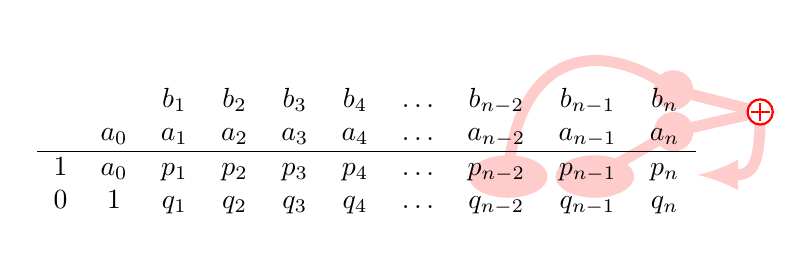
\begin{tikzpicture}[>=latex,thick]
\coordinate (c1) at (1.9,1.2);
\coordinate (c2) at (2.9,1.5);
\draw[color=red!20,line width=4pt] (1.8,-0.32) .. controls (c1) and (c2) .. (3.9,0.78);
\draw[color=red!20,line width=4pt] (2.9,-0.32) -- (3.9,0.25);
\draw[color=red!20,line width=4pt] (3.9,0.25) -- (5,0.5);
\draw[color=red!20,line width=4pt] (3.9,0.78) -- (5,0.5);

\begin{scope}[xshift=1.8cm,yshift=-0.32cm]
\fill[color=red!20] (0.0,0) ellipse (0.50cm and 0.27cm);
\end{scope}


\begin{scope}[xshift=2.9cm,yshift=-0.32cm]
\fill[color=red!20] (0.0,0) ellipse (0.50cm and 0.27cm);
\end{scope}

\begin{scope}[xshift=3.9cm,yshift=0.78cm]
\fill[color=red!20] (0,0) ellipse (0.25cm and 0.25cm);
\end{scope}

\begin{scope}[xshift=3.9cm,yshift=0.25cm]
\fill[color=red!20] (0,0) ellipse (0.25cm and 0.25cm);
\end{scope}

\begin{scope}[xshift=5.0cm,yshift=0.5cm]
\draw[->,color=red!20,line width=4pt]
	(0,0) .. controls (0,-0.7) and (-0.1,-0.8) .. (-0.8,-0.8);
\fill[color=white] (0,0) circle[radius=0.16];
\draw[color=red] (0,0) circle[radius=0.16];
\draw[color=red] (-0.12,0)--(0.12,0);
\draw[color=red] (0,-0.12)--(0,0.12);
\end{scope}
\node at (0,0) {\begin{tabular}{>{$}c<{$}>{$}c<{$}>{$}c<{$}>{$}c<{$}>{$}c<{$}>{$}c<{$}>{$}c<{$}>{$}c<{$}>{$}c<{$}>{$}c<{$}}
        &     & b_1 & b_2 & b_3 & b_4 & \dots & b_{n-2} & b_{n-1} & b_n \\
        & a_0 & a_1 & a_2 & a_3 & a_4 & \dots & a_{n-2} & a_{n-1} & a_n \\
\hline
   1    & a_0 & p_1 & p_2 & p_3 & p_4 & \dots & p_{n-2} & p_{n-1} & p_n \\
   0    &  1  & q_1 & q_2 & q_3 & q_4 & \dots & q_{n-2} & q_{n-1} & q_n \\
\end{tabular}};
\end{tikzpicture}
\end{center}
Die Berechung von $p_n$ aus $p_{n-2}$, $p_{n-1}$ und den Koeffizienten
$b_n$ und $a_n$ ist rot hervorgehoben, die Berechnung von $q_n$ erfolgt
nach dem gleichen Muster.

Für einen regulären Kettenbruch vereinfachen sich wegen $b_k=1$ die
Rekursionsformeln \eqref{eqn:cf:rekursion2} zu
\begin{equation}
\begin{aligned}
p_n&= p_{n-2} + p_{n-1}a_n\\
q_n&= q_{n-2} + q_{n-1}a_n
\end{aligned}
\label{eqn:cf:rekursion3}
\end{equation}
und im Berechnungsschema kann man sich ebenfalls die oberste Zeile
einsparen.
\begin{center}
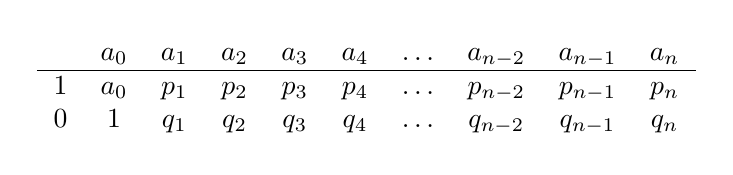
\begin{tikzpicture}[>=latex,thick]
\node at (0,0) {\begin{tabular}{>{$}c<{$}>{$}c<{$}>{$}c<{$}>{$}c<{$}>{$}c<{$}>{$}c<{$}>{$}c<{$}>{$}c<{$}>{$}c<{$}>{$}c<{$}}
        & a_0 & a_1 & a_2 & a_3 & a_4 & \dots & a_{n-2} & a_{n-1} & a_n \\
\hline
   1    & a_0 & p_1 & p_2 & p_3 & p_4 & \dots & p_{n-2} & p_{n-1} & p_n \\
   0    &  1  & q_1 & q_2 & q_3 & q_4 & \dots & q_{n-2} & q_{n-1} & q_n \\
\end{tabular}};
\end{tikzpicture}
\end{center}

\begin{beispiel}
Man berechne die Näherungsbrüche für den regulären Kettenbruch
\[
\pi
=
[3; 7, 15, 1, 292, 1, 1, 1, 2, 1, 3, 1, 14, 2, 1, 1,\dots].
\]
Das oben eingeführte Berechnungsschema ergibt:
\begin{center}
\begin{tabular}{
>{$}r<{$}
>{$}r<{$}
>{$}r<{$}
>{$}r<{$}
>{$}r<{$}
>{$}r<{$}
>{$}r<{$}
>{$}r<{$}
>{$}r<{$}
>{$}r<{$}
>{$}r<{$}}
 & 3&  7&  15&   1&    292&      1&      1&      1&      2&       1\\
\hline
1& 3& 22& 333& 355& 103993& 104348& 208341& 312689& 833719& 1146408\\
0& 1&  7& 106& 113&  33102&  33215&  66317&  99532& 265381&  364913\\
\hline
\end{tabular}
\end{center}
Man kann daraus die folgenden Näherungsbrüche für $\pi$ ablesen,
die korrekten Stellen in der Dezimaldarstellung sind unterstrichen:
\[
\begin{aligned}
\frac{p_0}{q_0}&=\frac{      3}{     1}
	&&=\underline{3}.00000000000000000000\\
\frac{p_1}{q_1}&=\frac{     22}{\phantom{0}7}
	&&=\underline{3}.\underline{14}285714285714285714\\
\frac{p_2}{q_2}&=\frac{    333}{   106}
	&&=\underline{3}.\underline{1415}0943396226415094\\
\frac{p_3}{q_3}&=\frac{    355}{   113}
	&&=\underline{3}.\underline{141592}92035398230088\\
\frac{p_4}{q_4}&=\frac{ 103993}{\phantom{0}33102}
	&&=\underline{3}.\underline{141592653}01190260407\\
\frac{p_5}{q_5}&=\frac{ 104348}{\phantom{0}33215}
	&&=\underline{3}.\underline{141592653}92142104470\\
\frac{p_6}{q_6}&=\frac{ 208341}{\phantom{0}66317}
	&&=\underline{3}.\underline{141592653}46743670552\\
\frac{p_7}{q_7}&=\frac{ 312689}{\phantom{0}99532}
	&&=\underline{3}.\underline{141592653}61893662339\\
\frac{p_8}{q_8}&=\frac{ 833719}{265381}
	&&=\underline{3}.\underline{1415926535}8107777120\\
\frac{p_9}{q_9}&=\frac{1146408}{\phantom{0}364913}
	&&=\underline{3}.\underline{14159265359}140397848\\
\end{aligned}
\]
\end{beispiel}



